\documentclass[parskip=full]{article}
\usepackage[utf8]{inputenc}
\usepackage{amsthm, amssymb, mathtools, esdiff,stmaryrd, tcolorbox, bbm,float, physics}
\usepackage{tikz-cd}
\usepackage{algorithm, pdfpages}
\usepackage{bm, url, booktabs}
\usepackage[noend]{algpseudocode}
\usepackage{listings}
\usepackage{xcolor}
\usepackage[left=1.5cm, right=1.5cm]{geometry}
\usepackage{lipsum}
\usepackage{subfig}
\usepackage{hyperref}
\usepackage[nameinlink]{cleveref}
\hypersetup{
    colorlinks=true,
    linkcolor=blue,
    filecolor=magenta,      
    urlcolor=cyan,
    pdftitle={Overleaf Example},
    pdfpagemode=FullScreen,
    }

\title{Measure theory notes}
\author{jyl20 }
\date{February 2022}
\newtheorem{theorem}{Theorem}[section]
\theoremstyle{definition}
\newtheorem*{definition}{Definition}
\newtheorem{corollary}{Corollary}
\newtheorem{proposition}{Proposition}[section]
\newtheorem{lemma}{Lemma}[proposition]
\newtheorem*{proofsketch}{Sketch of proof}
\newtheorem{problem}{Problem}[section]
\newtheorem*{solution}{Solution}
\newtheorem*{remark}{Remark}
\newtheorem*{example}{Example}
\setlength{\parindent}{0pt}
\DeclareMathOperator*{\argmax}{arg\,max}
\DeclareMathOperator*{\argmin}{arg\,min}
\newlength{\NOTskip} 
\renewcommand{\d}[1]{\ensuremath{\operatorname{d}\!{#1}}}
\newcommand*\interior[1]{\mathring{#1}}
\newcommand*\closure[1]{\overline{#1}}
\newcommand{\R}{\mathbb{R}}
\newcommand{\Rbar}{\overline{\R}}
\newcommand{\lsup}{\limsup_{n \to \infty}}
\newcommand{\linf}{\liminf_{n \to \infty}}
\newcommand{\ceq}{\coloneqq}
\newcommand{\limn}{\lim_{n\to \infty}}
\newcommand{\mn}{m\geq n}
\newcommand{\xseq}{(x_n)_{n \in \mathbb{N}}}
\newcommand{\setseq}{(A_n)_{n \in \mathbb{N}}}
\newcommand{\setunion}{\cup_{n \in \mathbb{N}}(A_n)}
\newcommand{\N}{\mathbb{N}}
\newcommand{\Q}{\mathbb{Q}}
\newcommand{\intm}[2][X]{\int_#1 #2 \, d \mu}
\newcommand{\sumlim}{\sum_{n=1}^\infty}
\newcommand{\measurablespace}{(\Omega, \mathcal{F})}
\newcommand{\measurespace}{(\Omega, \mathcal{F}, \mu)}
\newcommand{\F}{\mathcal{F}}
\newcommand{\C}{\mathcal{C}}
\newcommand{\G}{\mathcal{G}}
\newcommand{\B}{\mathcal{B}}
\newcommand{\I}{\mathcal{I}}
\newcommand{\Scal}{\mathcal{S}}
\newcommand{\Ccal}{\mathcal{C}}
\newcommand{\Lcal}{\mathcal{L}}
\newcommand{\A}{\mathcal{A}}
\newcommand{\Pbb}{\mathbb{P}}
\newcommand{\Pcal}{\mathcal{P}} 
\newcommand{\bracketsigma}{($\sigma$-)}
\newcommand{\probabilityspace}{(\Omega,\F,\Pbb)}
\newcommand{\1}{\mathbbm{1}}
\newcommand{\Var}{\mathrm{Var}}
\newcommand{\E}{\mathbb{E}}
\setlength{\parskip}{1\baselineskip plus 2pt}

\lstset{
breaklines=true,
}

\begin{document}
Throughout, let $(\Omega, \F, \Pbb)$ be a probability space.
\section{Conditional expectation}
\begin{theorem}[Existence and uniqueness of conditional expectation]
  Let $X \in L^1$, and $\mathcal{G} \subseteq \mathcal{F}$. Then there exists a random variable $Y$ such that
  \begin{itemize}
    \item $Y$ is $\mathcal{G}$-measurable
    \item $Y \in L^1$, and $\E X \mathbf{1}_A = \E Y \mathbf{1}_A$ for all $A \in \mathcal{G}$.
  \end{itemize}

  Moreover, if $Y'$ is another random variable satisfying these conditions, then $Y' = Y$ almost surely.

  We call $Y$ a (version of) the conditional expectation given $\mathcal{G}$.
\end{theorem}

\begin{proof}(Existence)

  Case 1: $X \in L^2$.

  Recall that $L^2$ is a Hilbert space, and that the set of $\mathcal{G}$-measurable random variables is a closed subspace of $L^2$ (it is closed because the space $L^2(\Omega, \mathcal{G}, \Pbb)$ is complete). The projection theorem then gives us the existence and uniqueness of $Y\in L^2 \subseteq L^1$.

  Case 2: $X \geq 0 \in L^1$.

  Let $X_n = X \wedge n \in L^2$. Then by case 1, we can define $Y_n = \E(X_n \mid \mathcal{G}) \in L^2$. We make the following observation

  \begin{lemma}
    Suppose $(X, Y)$ and $(X', Y')$ are two pairs of random variables satisfying the conditions of the theorem, then $X \geq X'$ implies $Y \geq Y'$ almost surely.
  \end{lemma}

  \begin{proof}
    Let $A = \{Y < Y'\}$. Then $\E Y \mathbf{1}_A = \E X \mathbf{1}_A \geq \E X' \mathbf{1}_A = \E Y' \mathbf{1}_A$, so $\E (Y - Y') \mathbf{1}_A \geq 0$ and $\Pbb(A) = 0$.
  \end{proof}

  It follows that there is some random variable $Y$ such that $Y_n \uparrow Y$. Clearly $Y$ is $\mathcal{G}$-measurable. For any $A \in \mathcal{G}$, we have
  \begin{align*}
    \E Y \mathbf{1}_A & = \lim_{n \to \infty} \E Y_n \mathbf{1}_A &   & \text{(MCV)} \\
                      & = \lim_{n \to \infty} \E X_n \mathbf{1}_A &   & \text{(MCV)} \\
    &= \E X \mathbf{1}_A
  \end{align*}

  Case 3: $X \in L^1$.

  Write $X = X^+ - X^-$, and apply case 2 to $X^+$ and $X^-$.

  (Uniqueness)
  Suppose $Y$ and $Y'$ are two random variables satisfying the conditions of the theorem. The $\{Y > Y'\}$ is in $\mathcal{G}$ so $\E Y \mathbf{1}_{\{Y > Y'\}} = \E Y' \mathbf{1}_{\{Y > Y'\}} \implies \E (Y - Y') \mathbf{1}_{\{Y > Y'\}} = 0 \implies \Pbb(Y > Y') = 0$. Similarly, $\Pbb(Y' > Y) = 0$.


  \begin{remark}
    The above can also be proved using the Radon-Nikodym theorem.
  \end{remark}

  (Proof via Radon-Nikodym)
  First recall the Radon-Nikodym theorem
  \begin{proposition}[Radon-Nikodym theorem]
    Let $\mu, \nu$ be two $\sigma$-finite measures on $(\Omega, \mathcal{F})$ such that $\nu \ll \mu$. Then there exists a unique (up to a.e. equivalence) $f \in L^1(\Omega, \mathcal{F}, \mu)$ such that $\nu(A) = \int_A f \, d\mu$ for all $A \in \mathcal{F}$.
  \end{proposition}
  Consider the measure on $(\Omega, \mathcal{G})$ given by
  \[
    \mu(A) = \E X \mathbf{1}_A, \quad A \in \mathcal{G}
  \]
  so $\mu \ll \Pbb$. By the Radon-Nikodym theorem, there exists a unique $Y \in L^1(\Omega, \mathcal{G}, \Pbb)$ such that $\mu(A) = \int_A Y \, d\Pbb$ for all $A \in \mathcal{G}$.

  For general $X \in L^1$, we can write $X = X^+ - X^-$ and apply the above to $X^+$ and $X^-$.
\end{proof}

\begin{proposition}[Equivalent definition for conditional expectation]
  Let $X, \mathcal{G}$ be as above. Then there exists a random variable $Y$ such that
  \begin{itemize}
    \item $Y$ is $\mathcal{G}$-measurable
    \item $Y \in L^1$ and $\E X Z = \E Y Z$ for all $Z \in L^\infty(\mathcal{G})$
  \end{itemize}

  Moreover, $Y = \E(X \mid \mathcal{G})$ almost surely.
\end{proposition}

\begin{proof}
  (Existence)
  Set $Y = \E(X \mid \mathcal{G})$. It is straightforward to see that $Y$ satisfies the conditions of the proposition for simple functions $Z$. Note that simple functions that are in $L^p$ are dense in $L^p$ for $1 \leq p \leq \infty$. Let $Z_n \in L^\infty(\mathcal{G})$ be a sequence of simple functions such that $Z_n \to Z$ in $L^\infty$ (in particular, we have almost sure pointwise convergence). Then
  \begin{align*}
    \E X Z & = \lim_{n \to \infty} \E X Z_n &   & \text{(DCT)} \\
    &= \lim_{n \to \infty} \E Y Z_n\\
           & = \E Y Z                       &   & \text{(DCT)}
  \end{align*}
\end{proof}

(Uniqueness) Note that any two random variables satisfying the conditions of the proposition are versions of the conditional expectation given $\mathcal{G}$, which was shown to be unique.

\begin{lemma}[Conditional expectation as a function]
  Let $X, Y: (\Omega, \F) \to (\R, \B(\R))$. Then $Y$ is measurable with respect to $\sigma(X)$ if and only if there exists a Borel-measurable function $f: \R \to \R$ such that $Y(\omega) = f(X(\omega))$ for all $\omega \in \Omega$.
\end{lemma}


\begin{proposition}[Properties of conditional expectation]
  All (in)equality relations below hold almost surely.
  \begin{enumerate}
    \item If $X \geq 0$ a.s., then $\E(X \mid \mathcal{G}) \geq 0$
    \item If $X$ and $\mathcal{G}$ are independent, then $\E(X \mid \mathcal{G}) = \E[X]$
    \item If $\alpha, \beta \in \R$ and $X_1, X_2 \in L^1$, then
          \[
            \E(\alpha X_1 + \beta X_2 \mid \mathcal{G}) = \alpha \E(X_1 \mid\mathcal{G}) + \beta \E(X_2 \mid \mathcal{G}).
          \]
    \item \emph{Tower property}\index{tower property}: If $\mathcal{H} \subseteq \mathcal{G}$, then
          \[
            \E(\E(X \mid \mathcal{G}) \mid \mathcal{H}) = \E(X \mid \mathcal{H}).
          \]
    \item If $Z$ is bounded and $\mathcal{G}$-measurable, then
          \[
            \E(ZX \mid \mathcal{G}) = Z \E(X \mid \mathcal{G}).
          \]
    \item Let $X \in L^1$ and $\mathcal{G}, \mathcal{H} \subseteq \mathcal{F}$. Assume that $\sigma(X, \mathcal{G})$ is independent of $\mathcal{H}$. Then
          \[
            \E (X \mid \mathcal{G}) = \E(X \mid \sigma(\mathcal{G}, \mathcal{H})).
          \]
  \end{enumerate}
\end{proposition}

\begin{proof}
  \begin{enumerate}
    \item Follows from the proof of existence and uniqueness of conditional expectation, or just use monotonicity.
    \item Let $A \in \mathcal{G}$. Then $\E( \E(X) \mathbf{1}_A) = \E X \E 1_A = \E (X 1_A)$
    \item Use linearity of conditional expectation.
    \item Let $A \in \mathcal{H}$. Then $\E\left[\E(\E(X \mid \mathcal{G}) \mid \mathcal{H}) \mathbf{1}_A \right] = \E [\E(X \mid \mathcal{G}) \mathbf{1}_A] = \E(X \mathbf{1}_A)$
    \item Easy if $Z$ is an indicator function. Then use linearity and covergence theorems.
    \item Note $\E (X \mid \mathcal{G})$ is $\sigma(\mathcal{G}, \mathcal{H})$-measurable and $\sigma(\mathcal{G}, \mathcal{H})$ is generated by the $\pi$-system $\{A \cap B: A \in \mathcal{G}, B \in \mathcal{H}\}$. We show that $\E(X \mid \mathcal{G})$ satisfies the defining property of $\E(X \mid \sigma(\mathcal{G}, \mathcal{H}))$. Let $A \in \mathcal{G}$ and $B \in \mathcal{H}$. Then for any element of the $\pi$-system, we have
          \[
            \E(\E(X \mid \mathcal{G}) \mathbf{1}_{A \cap B}) = \E [\E(X \mid \mathcal{G}) \mathbf{1}_A \mathbf{1}_B] = \E [\E(X \mathbf{1}_A \mid \mathcal{G}) \mathbf{1}_B] = \E(\underbrace{X \mathbf{1}_A}_{\in \sigma(\mathcal{G}, X)}) \E(\mathbf{1}_B) = \E(X \mathbf{1}_{A \cap B})
          \]
          Since finite measures extend uniquely from $\pi$-systems, the above holds if $A\cap B$ is replaced by any element of $\sigma(\mathcal{G}, \mathcal{H})$
  \end{enumerate}
\end{proof}

\begin{proposition}[Properties of conditional expectation] 
  \label{Properties of conditional expectation}
  All (in)equality relations below hold almost surely.
  \begin{enumerate}
    \item \emph{Jensen's inequality}: If $c: \R \to \R$ is convex, then
          \[
            \E(c(X) \mid \mathcal{G}) \geq c(\E(X \mid \mathcal{G})).
          \]
    \item \emph{Conditional expectation is a contraction} For $p \geq 1$,
          \[
            \|\E(X \mid \mathcal{G})\|_p \leq \|X\|_p.
          \]
    \item \emph{Monotone convergence theorem} Suppose $X_n \uparrow X$ is a sequence of non-negative random variables. Then
          \[
            \E(X_n\mid \mathcal{G}) \uparrow \E(X \mid \mathcal{G}).
          \]
    \item \emph{Fatou's lemma}: If $X_n$ are non-negative measurable, then
          \[
            \E\left(\liminf_{n \to \infty} X_n \mid \mathcal{G}\right) \leq \liminf_{n \to \infty} \E(X_n \mid \mathcal{G}).
          \]
    \item \emph{Dominated convergence theorem}\index{dominated convergence theorem}: If $X_n \to X$ and $Y \in L^1$ such that $Y \geq |X_n|$ for all $n$, then
          \[
            \E(X_n \mid \mathcal{G}) \to \E(X \mid \mathcal{G}).
          \]
  \end{enumerate}
\end{proposition}

\begin{proof}
  \begin{enumerate}
    \item Note that a convex function is the supremum of countably many affine functions $c(x) = \sup_{i \in I} a_i x + b_i$. Then
          \begin{align*}
            \E(c(X) \mid \mathcal{G}) &= \E \left(\sup_{i \in I}\left( a_i X + b_i \right)\mid \mathcal{G} \right)\\
              & \geq \E(a_i X + b_i \mid \mathcal{G}) \quad \forall i \in I &   & \text{(monotonicity)} \\
          \end{align*}
          So $\E(c(X) \mid \mathcal{G}) \geq \sup_{i \in I} \E(a_i X + b_i \mid \mathcal{G}) = c(\E(X \mid \mathcal{G}))$.
    \item Jensen
    \item By monotonicity, $\E(X_n \mid \mathcal{G}) \uparrow Y$ for some $Y$. By the usual monotone convergence theorem, $\E \E (X_n \mid \mathcal{G}) = \E X_n \to \E Y \leq \E X$ so $Y \in L^1$. Since each of the $\E (X_n \mid \mathcal{G})$ are $\mathcal{G}$-measurable, so is $Y$. Finally, for any $A \in \mathcal{G}$,
          \begin{align*}
            \E Y \mathbf{1}_A & = \lim_{n \to \infty} \E \E(X_n \mid \mathcal{G}) \mathbf{1}_A &   & \text{(MCV)} \\
            &= \lim_{n \to \infty} \E X_n \mathbf{1}_A\\
                              & = \E X \mathbf{1}_A                                            &   & \text{(MCV)}
          \end{align*}
    \item \begin{align*}
            \E \left (\liminf_{n \to \infty} X_n \mid \mathcal{G} \right) &= \E \left (\lim_{n \to \infty} \underbrace{\inf_{m \geq n} X_m}_{increasing} \mid \mathcal{G} \right)\\
              & = \lim_{n \to \infty} \E \left (\inf_{m \geq n} X_m \mid \mathcal{G} \right) &   & \text{(MCV)}          \\
            &= \liminf_{n \to \infty} \E \left (\underbrace{\inf_{m \geq n} X_m}_{\leq X_n} \mid \mathcal{G}\right)\\
              & \leq \liminf_{n \to \infty}\E(X_n \mid \mathcal{G})                          &   & \text{(monotonicity)}
          \end{align*}
    \item Use Fatou's lemma on $Y + X_n$ and $Y - X_n$.
  \end{enumerate}
\end{proof}

\section{Martingales}
\begin{definition}[(Discrete) stochastic process]
  A \emph{stochastic process} (in discrete time) is a collection of random variables $(X_n)_{n \in \mathbb{N}}$. A stochastic process is is \emph{integrable} if $X_n \in L^1$ for all $n$.
\end{definition}
\begin{definition}[Filtration]
  A \emph{filtration} is a sequence of $\sigma$-algebras $\mathcal{F}_n \subseteq \mathcal{F}$ such that $\mathcal{F}_n \subseteq \mathcal{F}_{n+1}$ for all $n$. We define $F_\infty = \sigma(\bigcup_{n=1}^\infty \mathcal{F}_n).$ The \emph{natural filtration} of a stochastic process $X$ is the filtration $\mathcal{F}_n = \sigma(X_1, \ldots, X_n)$. A stochastic process is \emph{adapted} to a filtration $\mathcal{F}_n$ if $X_n$ is $\mathcal{F}_n$-measurable for all $n$.
\end{definition}

\begin{definition}[Martingale]
  An integrable adapted process $(X_n)_{n \geq 0}$ is a \emph{martingale} if for all $n \geq m$, we have
  \[
    \E(X_n \mid \mathcal{F}_m) = X_m.
  \]
  We say it is a \emph{super-martingale} if
  \[
    \E(X_n \mid \mathcal{F}_m) \leq X_m,
  \]
  and a \emph{sub-martingale} if
  \[
    \E(X_n \mid \mathcal{F}_m) \geq X_m,
  \]
\end{definition}
By the tower property, it is sufficient to check the martingale property for $n = m+1$.

\begin{theorem}[Doob decomposition, non-examinable]
  Let $X_n$ be an integrable adapted process. Then there exists a martingale $M_n$ and an integrable predictable process $A_n$ such that $X_n = M_n + A_n$ and $A_0 = 0$, where predictable means that $A_n$ is $\mathcal{F}_{n-1}$-measurable for all $n \geq 1$. Moreover, $M_n$ and $A_n$ are unique up to a.s. equivalence.
\end{theorem}

\begin{proof}
  (Existence)
  Add up the `known' bits to get $A$ and the `surprises' to get $M$. Formally,
  \begin{align*}
    A_n & = A_{n-1} + \E(X_n \mid \mathcal{F}_{n-1}) - X_{n-1}                            \\
    M_n & = M_{n-1} + \underbrace{X_n - \E(X_n \mid \mathcal{F}_{n-1})}_{\text{surprise}}
  \end{align*}

  (Uniqueness) Let $X_n = M_n + A_n = M'_n + A'_n$. Then $M_n - M'_n = A'_n - A_n$ is $\mathcal{F}_{n-1}$-measurable. But $M_n - M'_n$ is a martingale, so $\E(M_n - M'_n \mid \mathcal{F}_{n-1}) = 0$ so $M_n = M'_n$ almost surely. Similarly, $A_n = A'_n$ almost surely.
\end{proof}

\begin{definition}[Stopping time]
  A random variable $T: \Omega \to \mathbb{N} \cup \{\infty\}$ is a \emph{stopping time} if $\{T \leq n\} \in \mathcal{F}_n$ for all $n$.
\end{definition}
In the discrete case, we can equivalently require that $\{T = n\} \in \mathcal{F}_n$ for all $n$.
\begin{definition}[$X_T$]
  Let $X$ be a stochastic process and $T$ a stopping time. Then $X_T: \Omega \to \R$ is defined by cases
  \[
    X_T(\omega) = \begin{cases}
      X_n(\omega) & T(\omega) = n      \\
      0           & T(\omega) = \infty
    \end{cases}
  \]
\end{definition}

\begin{definition}[Stopped $\sigma$-algebra]
  Let $T$ be a stopping time. Then the \emph{stopped $\sigma$-algebra} is
  \[
    \mathcal{F}_T = \{A \in \mathcal{F}: A \cap \{T \leq n\} \in \mathcal{F}_n \text{ for all } n\}.
  \]
\end{definition}

\begin{example}
  Let $N=\text{\# of times a random walk hits -5 before it first hits 10}$ and $T$ be the first time the random walk hits 10. $N$ is $\mathcal{F}_T$-measurable
\end{example}

\begin{definition}[Stopped process]
  Let $X$ be a stochastic process and $T$ a stopping time. Then the \emph{stopped process} is $X^T_n = X_{T \wedge n}$
\end{definition}

\begin{proposition}
  $ $
  \begin{enumerate}
    \item If $T, S, (T_n)_{n \geq 0}$ are all stopping times, then
          \[
            T \vee S, T \wedge S, \sup_n T_n, \inf T_n, \limsup T_n, \liminf T_n
          \]
          are all stopping times.
    \item $\mathcal{F}_T$ is a $\sigma$-algebra
    \item If $S \leq T$, then $\mathcal{F}_S \subseteq \mathcal{F}_T$.
    \item $X_T \mathbf{1}_{T < \infty}$ is $\mathcal{F}_T$-measurable.
    \item If $(X_n)$ is an adapted process, then so is $(X^T_n)_{n \geq 0}$ for any stopping time $T$.
    \item If $(X_n)$ is an integrable process, then so is $(X^T_n)_{n \geq 0}$ for any stopping time $T$.
  \end{enumerate}
\end{proposition}

\begin{proof}
  $ $
  \begin{enumerate}
    \item Elementary
    \item Elementary
    \item Let $A \in \mathcal{F}_S$. For any $n$, we have $A \cap \{S \leq n\} \in \mathcal{F}_n$ and $A \cap \{T \leq n\} = A \cap \{S \leq n\} \cap \{T \leq n\} \in \mathcal{F}_n$.
    \item $X_T \mathbf{1}_{T < \infty} = \sum_{n=1}^\infty X_n \mathbf{1}_{\{T = n\}}$ where each of the terms is $\mathcal{F}_T$-measurable.
    \item $X^T_n = X_n \mathbf{1}_{\{T \geq n\}} + X_T \mathbf{1}_{\{T < n\}} \mathbf{1}_{\{T < \infty\}}$.
    \item $X^T_n = X_n \mathbf{1}_{\{T \geq n\}} + \sum _{k=1}^{n-1} X_k \mathbf{1}_{\{T = k\}}$ so $E |X^T_n| \leq E|X_n| + \sum_{k=1}^{n-1} E|X_k| < \infty$.
  \end{enumerate}
\end{proof}

\begin{theorem}[Equivalent definitions for super-martingales]
  Let $(X_n)_{n \geq 0}$ be an integrable and adapted process. Then the following are equivalent:
  \begin{enumerate}
    \item $(X_n)_{n \geq 0}$ is a super-martingale.
    \item For any bounded stopping time $T$ and any stopping time $S$,
          \[
            \E(X_T \mid \mathcal{F}_S) \leq X_{S \wedge T}.
          \]
    \item $(X_n^T)$ is a super-martingale for any stopping time $T$.
    \item \label{super martingale: monotone} For bounded stopping times $S, T$ such that $S \leq T$, we have
          \[
            \E X_T \leq \E X_S.
          \]
  \end{enumerate}
\end{theorem}

\begin{proof}
  \begin{itemize}
    \item[--] $(2) \Rightarrow (1)$: Let $n \geq m$ and set $T = n, S = m$.
    \item[--] $(2) \Rightarrow (4)$: Tower rule
    \item[--] $(2) \Rightarrow (3)$: Let $n \geq m$
          \[
            \E(X_n^T \mid \mathcal{F}_m) = \E (X_{T \wedge n} \mid \mathcal{F}_m) \leq X_{T \wedge m \wedge n} = X_m^T.
          \]
    \item[--] $(1) \Rightarrow (2)$ Let $T \leq N$
          \begin{align*}
            X_T & =X_{S \wedge T} + \sum_{k = 0}^N (X_{k + 1} - X_k) \mathbf{1}_{S \leq k < T} \tag{$*$}
          \end{align*}
          Let $A \in \mathcal{F}_S$.
          \begin{align*}
            \E \left[(X_{k + 1} - X_k)\mathbf{1}_{S \leq k < T} \mathbf{1}_A \right] & = \E \left[\E \left[(X_{k + 1} - X_k)\underbrace{\mathbf{1}_{S \leq k < T}\mathbf{1}_A}_{\in \mathcal{F}_k} \mid \mathcal{F}_k \right]\right] \\
                                                                                     & = \E \left[ \mathbf{1}_{S \leq k < T} \mathbf{1}_A \underbrace{\E \left[(X_{k + 1} - X_k) \mid \mathcal{F}_k \right]}_{\leq 0}\right]         \\
                                                                                     & \leq 0
          \end{align*}
          so $\E X_T \mathbf{1}_A \leq \E X_{S \wedge T} \mathbf{1}_A$. By Radon-Nikodym, $\E(X_{S \wedge T} - X_T \mid \mathcal{F}_S) \geq 0$. But $X_{S \wedge T}$ is $\mathcal{F}_S$-measurable, so $X_{S \wedge T} - X_T \geq 0$ almost surely.

    \item[--] $(4) \Rightarrow (2)$ Let $n \geq m$ and $A \in \mathcal{F}_m$. One can check that $T = m \mathbf{1}_A + n \mathbf{1}_{A^c} \leq n$ is a stopping time such that
          \begin{align*}
            \E((X_n - X_m) \mathbf{1}_A) & = \E(X_n - X_T) \leq 0 \\
          \end{align*}
          By Radon-Nikodym, $\E(X_m - X_n \mid \mathcal{F}_m) \geq 0$ so $\E(X_n \mid \mathcal{F}_m) \leq X_m$.

    \item [--] $(3) \Rightarrow (1)$ Let $T = \infty$
  \end{itemize}
\end{proof}

\begin{proposition}[Convex transformations of martingales]
  Let $(X_n)$ be a martingale and $c: \R \to \R$ a convex function. Then $(c(X_n))$ is a sub-martingale.
\end{proposition}

\begin{proof}
  Let $S \leq T$ be bounded stopping times. Then
  \begin{align*}
    \E(c(X_T) \mid \mathcal{F}_S) & \geq c(\E(X_T \mid \mathcal{F}_S)) &   & \text{(Jensen)} \\
                                  & = c(X_S)                          
  \end{align*}
\end{proof}

\begin{theorem}[Optional stopping]
  Let $(X_n)_{n \geq 0}$ be a martingale and $T$ a stopping time. Then $E(X_T) = E(X_0)$ if any of the following conditions hold:
  \begin{enumerate}
    \item $T$ is almost surely bounded, i.e. there is some $N$ such that $T \leq N$ almost surely.
    \item $X$ has bounded increments, i.e. there is some $K$ such that $|X_{n+1} - X_n| \leq K$ for all $n$ almost surely and $T$ is integrable
    \item There exists an integrable random variable $Y$ such that $|X_n| \leq Y$ for all $n$ almost surely and $T$ is finite almost surely, i.e. $\Pbb(T < \infty) = 1$.
  \end{enumerate}
\end{theorem}

\begin{proof}
  \begin{enumerate}
    \item Use (\ref{super martingale: monotone}) of the previous theorem with $S = 0$, or prove directly.
    \item placeholder
    \item placeholder
  \end{enumerate}
\end{proof}

\section{Convergence}
\begin{definition}[Upcrossing]
  Let $(x_n)$ be a sequence and $(a, b)$ an interval. An \emph{upcrossing} of $(a, b)$ by $(x_n)$ is a sequence $j, j + 1, \ldots, k$ such that $x_j \leq a$ and $x_k \geq b$. We define\index{$U_n[a, b, (x_n)]$}\index{$U[a, b, (x_n)$}
  \begin{align*}
    U_n[a, b, (x_n)] & = \text{number of disjoint upcrossings contained in }\{1, \ldots, n\} \\
    U[a, b, (x_n)]   & = \lim_{n \to \infty} U_n[a, b, (x_n)].
  \end{align*}
\end{definition}

\begin{figure*}[h]
  \centering
  \includegraphics*{upcrossings.png}
  \caption{Three upcrossings. \href{https://almostsuremath.com/2009/12/06/upcrossings-downcrossings-and-martingale-convergence/}{Source}}
\end{figure*}

The notion of upcrossings is related to the notion of convergence.

\begin{proposition}
  A sequence $(x_n)$ converges to a limit in the extended real numbers if and only if $U[a, b, (x_n)] < \infty$ for all rationals $a < b$.
\end{proposition}

\begin{proposition}[Doob's upcrossing inequality]
  Let $X=(X_k)$ be a super-martingale and $a < b$. Then
  \[
    (b - a) \E U_n[a, b, X] \leq \E[(X_n - a)^-].
  \]
\end{proposition}

\begin{proof}
  Assume that $X$ is a super-martingale. We define stopping times $S_k, T_k$ as follows:
  \begin{itemize}
    \item $T_0 = 0$
    \item $S_{k + 1} = \inf\{n: X_n \leq a, n \geq T_n\}$
    \item $T_{k + 1} = \inf\{n: X_n \geq b, n \geq S_{k + 1}\}$.
  \end{itemize}\
  Note that the times alternate, i.e.  $S_k \leq T_k \leq S_{k + 1} \leq T_{k + 1}$

  The idea is to sum up the increments of each upcrossing. Consier the set $\mathcal{I} \coloneqq \{k: S_k < T_k < n\}$ and the sum
  \[
    \underbrace{\sum_{k \in \mathcal{I}} (X_{T_k} - X_{S_k})}_{\geq (b - a)U_n[a, b, X]} + \begin{cases}
      X_n - X_{S_{\max \mathcal{I} + 1}} & \text{if } n > S_{\max \mathcal{I} + 1} \\
      0                                  & \text{otherwise}
    \end{cases}
  \]


  \begin{figure}[h]
    \centering
    \subfloat[No extra term]{
      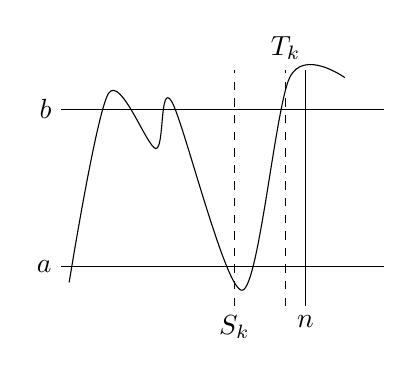
\begin{tikzpicture}
        \draw (-0.1, 0) node [left] {$b$} -- (4, 0);
        \draw (-0.1, -2) node [left] {$a$} -- (4, -2);
        \draw (3, -2.5) node [below] {$n$} -- (3, 0.5);
        \draw [dashed] (2.1, -2.5) node [below] {$S_k$} -- (2.1, 0.5);
        \draw [dashed] (2.75, -2.5) -- (2.75, 0.5) node [above] {$T_k$};
        \draw plot [smooth] coordinates {(0, -2.2) (0.5, 0.2) (1.1, -0.5) (1.3, 0.1) (2.2, -2.3) (2.8, 0.4) (3.5, 0.4)};
      \end{tikzpicture}
    }
    \qquad
    \subfloat[Extra term]{
      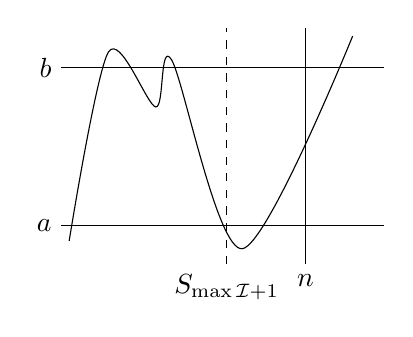
\begin{tikzpicture}
        \draw (-0.1, 0) node [left] {$b$} -- (4, 0);
        \draw (-0.1, -2) node [left] {$a$} -- (4, -2);
        \draw (3, -2.5) node [below] {$n$} -- (3, 0.5);
        \draw [dashed] (2, -2.5) node [below] {$S_{\max \mathcal{I} + 1}$} -- (2, 0.5);
        \draw plot [smooth] coordinates {(0, -2.2) (0.5, 0.2) (1.1, -0.5) (1.3, 0.1) (2.2, -2.3) (3.6, 0.4)};
      \end{tikzpicture}
    }
      \caption{Graphs taken from \href{https://almostsuremath.com/2009/12/06/upcrossings-downcrossings-and-martingale-convergence/}{here}}
  \end{figure}

  Note that each term is of the form $X_U - X_V$ for some \emph{bounded} stopping times $U \geq V$. By the property of super-martingales, $\E(X_U - X_V) \leq 0$ so the sum is negative in expectation.

  Hence, 
  \begin{align*}
    (b - a) \E U_n[a, b, X] + \E(\underbrace{\underbrace{(X_n - X_{S_{\max \mathcal{I} + 1}})}_{
      \geq X_n - a \geq -(X_n - a)^-} \mathbf{1}_{n > S_{\max \mathcal{I} + 1}}}_{\geq -(X_n - a)^-}) &\leq 0 \\
    (b - a) \E U_n[a, b, X]  \leq  \E((X_n - a)^-) \leq \E(|X_n|) + |a|
  \end{align*}
\end{proof}

\begin{proposition}[Almost sure martingale convergence theorem] \label{almost sure martingale convergence theorem}
  Suppose $X = (X_n)_{n \geq 0}$ is a super-martingale that is bounded in $L^1$, i.e.\ $\sup_n \E|X_n| < \infty$. Then for any $a < b$, we have $U[a, b, X] < \infty$ almost surely. In particular, there exists an $\mathcal{F}_\infty$-measurable $X_\infty \in L^1$ such that
  \[
    X_n \to X_\infty\text{ a.s. as }n \to \infty.
  \]
\end{proposition}

\begin{remark}
  The intuition is that you cannot make money by betting on a super-martingale (without shorting). For any $a < b$, you can devise a betting strategy where you buy at $a$ and sell at $b$. If $U[a, b, X] = \infty$, then you make money almost surely.
\end{remark}

\begin{proof}
  Let $a < b$ and $n$ be arbitrary and $\sup_m \E|X_m| = M$. By Doob's upcrossing inequality, we have
  \begin{align*}
    (b - a) \E U_n[a, b, X] & \leq M + |a| < \infty \\
    (b - a) \E U[a, b, X] & \leq M + |a| < \infty && \text{(monotone convergence, $ U_n \uparrow U$)}
  \end{align*}
  So $U[a, b, X] < \infty$ almost surely.

  Now consider the set of events where $X_n$ converges
  \[
    A \coloneqq \cap_{a, b \in \Q} \{U[a, b, X] < \infty\}, \qquad \Pbb (A) = 1
  \]
  and define
  \[
    X_\infty = \begin{cases}
      \lim X_n & \text{on } A \\
      0           & \text{on } A^c
    \end{cases}
  \]
  which is $\mathcal{F}_\infty$-measurable. Note that $|X_\infty| = \liminf |X_n|$ almost surely and by Fatou's lemma,
  \[
    \E \liminf |X_n| \leq \liminf \E|X_n| \leq M < \infty.
  \]
  So $X_\infty \in L^1$.
\end{proof}

\begin{remark}
  Sone propositions below concern non-negative submartingales. Recall convex transformations, such as $|\cdot|$, turn a martinagle into a sub-martingale.
\end{remark}

\begin{proposition}[Doob's maximal inequality]
  Let $X = (X_n)_{n \geq 0}$ be a non-negative sub-martingale. Then for any $\lambda > 0$ and writing $X^*_n = \max_{0 \leq k \leq n} X_k$, we have
  \[
    \lambda \Pbb(X^*_n \geq \lambda) \leq \E X_n \mathbf{1}_{X^*_n \geq \lambda} \leq \E X_n.
  \]
\end{proposition}

\begin{proof}
  Let $T = \inf\{n: X_n \geq \lambda\}$
  \begin{align*}
    \E X_n \geq \E X_{T \wedge n} &= \E X_n \mathbf{1}_{T > n} + \E X_T \mathbf{1}_{T \leq n} \\
    \E X_n \mathbf{1}_{T \leq n} &\geq \lambda \Pbb(T \leq n) \\
    \E X_n \mathbf{1}_{X^*_n \geq \lambda} &\geq \lambda \Pbb(X^*_n \geq \lambda)
  \end{align*}
\end{proof}

\begin{corollary}
  Under the same hypotheses, let $X^*_n \uparrow X^*$. Then
  \[
    \lambda \Pbb(X^* \geq \lambda) \leq \sup_{n \geq 0} \E X_n
  \]
\end{corollary}

\begin{proposition}[Doob's $L^p$ inequality]
  Let $X = (X_n)_{n \geq 0}$ be a martingale or a non-negative sub-martingale. Then for any $p > 1$ and $n \geq 1$, we have
  \[
    \|X^*_n\|_p \leq \frac{p}{p - 1} \|X_n\|_p.
  \]
\end{proposition}

\begin{proof} (magic) \\
  Let $k > 0$ and $T = \inf\{n: X_n \geq k\}$. Then
  \begin{align*}
    \int |X_n^* \wedge k|^p \d \Pbb &= \int \left( 
      \int p x^{p - 1} \mathbf{1}_{\{0 \leq x \leq |X_n^* \wedge k|\}} \d x \right) \d \Pbb \\
      &= \int \left( 
        \int p x^{p - 1} \mathbf{1}_{\{|X_n^*| \geq x\}} \mathbf{1}_{\{0 \leq x \leq k\}} \d x \right) \d \Pbb \\
      & = \int p x^{p - 1} \Pbb(|X_n^*|\geq x) \mathbf{1}_{\{0 \leq x \leq k\}}\d x\\
      & \leq \int p x^{p - 1} \frac{1}{x} \E |X_n| \mathbf{1}_{\{|X_n^*| \geq x\}} \mathbf{1}_{\{0 \leq x \leq k\}} \d x &   & \text{(Doob's maximal inequality)} \\
      & = \int \int p x^{p - 2} |X_n| \mathbf{1}_{\{|X_n^*| \geq x\}} \mathbf{1}_{\{0 \leq x \leq k\}}\d x \d \Pbb \\
      & = \int \frac{p}{p - 1}  |X_n| (|X_n^*| \wedge k)^{p - 1} \d \Pbb \\
      & \leq \frac{p}{p - 1} \|X_n\|_p \| |X_n^*| \wedge k\|_p^{p - 1} &   & \text{(H\"older's inequality)} 
  \end{align*}

  By monotone convergence and taking $k \to \infty$, we get
  \[
    \|X_n^*\|_p^p \leq \frac{p}{p - 1} \|X_n\|_p \|X_n^*\|_p^{p - 1}
  \]
  and the result follows.
\end{proof}

\begin{corollary} \label{Doob Lp limit}
  Under the same hypotheses, let $X^*_n \uparrow X^*$. Then
  \[
    \|X^*\|_p \leq \frac{p}{p - 1} \sup_{n \geq 0} \|X_n\|_p
  \]
\end{corollary}

\begin{proposition}[Equivalent conditions for $L^p$ convergence, $p > 1$]
  Let $X = (X_n)_{n \geq 0}$ be a martingale, and $p > 1$. Then the following are equivalent:
  \begin{enumerate}
    \item $(X_n)_{n \geq 0}$ is bounded in $L^p$, i.e.\ $M = \sup_n \E |X_i|^p < \infty$.
    \item $(X_n)_{n \geq 0}$ converges as $n \to \infty$ to a random variable $X_\infty \in L^p$ almost surely and in $L^p$.
    \item There exists a random variable $Z \in L^p$ such that
      \[
        X_n = \E (Z \mid \mathcal{F}_n) \qquad \lim_{n \to \infty} X_n = \E (Z \mid \mathcal{F}_\infty) \text{ a.s.}
      \]
  \end{enumerate}
  This gives a bijection between martingales bounded in $L^p$ and $L^p(\mathcal{F}_\infty)$, sending $(X_n)_{n \geq 0} \mapsto X_\infty$.
\end{proposition}

\begin{proof}
  \begin{itemize}
    \item [--] $(1) \Rightarrow (2)$ By Jensen, $\E |X_n|^p \geq (\E |X_n| )^p$ so $X$ is bounded in $L^1$. By the almost sure martingale convergence theorem, there exists an $\mathcal{F}_\infty$-measurable $X_\infty \in L^1$ such that $X_n \to X_\infty$ almost surely. Note also $|X|^* \geq |X_n|$ for all $n$ and $X^* \in L^p$ by \Cref*{Doob Lp limit}. Hence, $X_n \to X_\infty$ in $L^p$ by $L^p$ dominated convergence

    \item [--] $(2) \Rightarrow (3)$ Let $Z = X_\infty$. Note $X_n \xrightarrow{L^p} X_\infty$ implies that $X$ is bounded in $L^p$. By Doob's maximal inequality, $|X|^* \in L^p \subseteq L^1$. By conditional dominated convergence, 
    \[
      \E (X_\infty \mid \mathcal{F}_n) = \lim_{m \to \infty} \E (X_m \mid \mathcal{F}_n) = X_n 
    \]

    \item [--] $(3) \Rightarrow (1)$ Conditional expectation is a contraction (\Cref*{Properties of conditional expectation})
  \end{itemize}
\end{proof}

\begin{definition}[Closed martingale]
  A martingale in the form $X_n = \E (Z \mid \mathcal{F}_n)$ for some $Z \in L^p$ is called a \emph{martingale closed in $L^p$}
\end{definition}

\begin{definition}[Non-examinable, uniform integrability for general measure space]
  Let $(f_n)_n$ be a family of absolutely integrable functions on some measure space. The family is said to be \emph{uniformly integrable (UI)} if all of the following hold
  \begin{enumerate}
    \item Uniform bound on $L^1$ norm ($\sup_n \int |f_n| < \infty$)
    \item No escape to vertical infinity ($\sup_n \int_{\{|f_n| > \lambda\}} |f_n| \to 0$ as $\lambda \to \infty$)
    \item No escape to horizontal infinity (for any $\varepsilon > 0$, there exists a finite measure subset $A$ such that $\sup_n \int_{A^c} |f_n| < \varepsilon$)
  \end{enumerate}
\end{definition}

\begin{example}
  A single integrable function is uniformly integrable. 
\end{example}

\begin{example}
  A family of functions which is dominated by some integrable function, i.e. there is $g \in L^1$ such that $|f_i| \leq g$ for all $i \in \mathcal{I}$, is uniformly integrable.
  \end{example}

\begin{definition}[Uniform integrability for random variables]
  A family of random variables $(X_i)_{i \in \mathcal{I}}$ is \emph{uniformly integrable} if
  \[
    \sup_{i \in \mathcal{I}} \E(|X_i| \mathbf{1}_{|X_i| > \alpha}) \to 0 \text{ as } \alpha \to \infty.
  \]
\end{definition}

\begin{remark}
  In the finite measure case, functions cannot escape to horizontal infinity and the conditions simplifies just to no escape to vertical infinity.
\end{remark}

\begin{figure}[h]
  \centering
  \begin{tikzpicture}[domain=0:4]
    \draw[->] (-0.2,0) -- (4.2,0) node[right] {$x$};
    \draw[->] (0,-1.2) -- (0,4.2) node[above] {$f(x)$};
  
    \draw (0, 1) node [left] {$1$} -- (4, 1);
    \draw [dashed] (4, 1) -- (4, 0) node [below] {$1$};
    \draw (0, 2) node [left] {$2$} -- (2, 2);
    \draw [dashed] (2, 2) -- (2, 0) node [below] {$2$};
    \draw (0, 3) node [left] {$n$} -- (1.33, 3);
    \draw [dashed] (1.33, 3) -- (1.33, 0) node [below] {$n$};
  \end{tikzpicture}
  \caption{Non uniformly integrable sequence}
\end{figure}

\begin{proposition}[Equivalent definition of uniform integrability]
  A family of random variables $(X_i)_{i \in \mathcal{I}}$ is \emph{uniformly integrable} if and only if both of the following hold
  \begin{enumerate}
    \item It is bounded in $L^1$ ($\sup_{i \in \mathcal{I}} \E(|X_i|) < \infty$)
    \item It is equi-integrable (For any $\varepsilon > 0$, there exists a $\delta > 0$ such that for any $A \in \mathcal{F}$ with $\Pbb(A) < \delta$, we have
    \[
      \E(|X_i| \mathbf{1}_A) < \varepsilon.
    \]
    for all $i \in \mathcal{I}$.)
  \end{enumerate}
\end{proposition}

\begin{theorem}[Non-examinable, Vitali convergence theorem]
  Let $f_1, f_2, \ldots$ be a sequence of integrable functions on some measure space and $1 \leq p < \infty$. Then $f_n \xrightarrow{L^p} f$ for some measurable $f$ if and only if all of the following hold
  \begin{enumerate}
    \item $(f_n^p)$ is uniformly integrable
    \item $f_n \to f$ in measure
    \item The sequence cannot escape to horizontal infinity, i.e.\ for any $\varepsilon > 0$, there exists a finite measure subset $A$ such that $\sup_n \int_{A^c} |f_n|^p < \varepsilon$.
  \end{enumerate}
\end{theorem}

\begin{remark}
  In the finite measure case, the third condition is trivially true and almost sure convergence implies convergence in measure, so this implies the $L^p$ dominated convergence theorem.
\end{remark}

\begin{proposition}[Conditional expectations are uniformly integrable] \label{Conditional expectations are uniformly integrable}
  Let $\mathcal{S}$ be a uniformly integrable family of random variables. Then the following set is uniformly integrable
  \[
    \mathcal{S}^* = \{\E(X|\mathcal{G}) \mid X \in \mathcal{S},\mathcal{G} \text{ is a sub $\sigma$-algebra of } \mathcal{F}\}.
  \]
\end{proposition}

\begin{proof}
  Since $\mathcal{S}$ is bounded in $L^1$, $\mathcal{S}^*$ is bounded in $L^1$. Let $\varepsilon > 0$. By uniform integrability of $\mathcal{S}$, there exists $\delta > 0$ such that for any $A \in \mathcal{F}$ with $\Pbb(A) < \delta$, we have $\E(|X| \mathbf{1}_A) < \varepsilon$ for all $X \in \mathcal{S}$. Note
  \[
    \E(|\E(X \mid \mathcal{G})|\mathbf{1}_A) \underbrace{\leq}_{Jensen} \E(\E (|X| \mid \mathcal{G})\mathbf{1}_A)
  \]
  we wish to show that when $A$ is of the form $\{|X| > \alpha\}$, the right hand side converges to zero as $\alpha \to \infty$. The right hand side becomes
$
    \E|X| \mathbf{1}_{\{|X| > \alpha\}}
$
  
  We want to choose $\alpha$ such that $\Pbb(|X| > \alpha) < \delta$. By Markov's inequality, 
  \[
    \Pbb(|X| > \alpha) \leq \frac{\E|X|}{\alpha}
  \]
  so picking any $\alpha > \frac{\E|X|}{\delta}$ works.

  We have shown that for any $\varepsilon > 0$, for any $\alpha$ sufficiently large, $\E(\left|\E(X \mid \mathcal{G})\right|\mathbf{1}_{\{|X|>\alpha\}}) \leq \varepsilon$
\end{proof}

\begin{proposition}[Equivalent conditions for $L^1$ convergence] \label{Equivalent conditions for L1 convergence}
  Let $(X_n)_{n \geq 0}$ be a martingale. Then the following are equivalent:
  \begin{enumerate}
    \item $(X_n)_{n \geq 0}$ is uniformly integrable.
    \item $(X_n)_{n \geq 0}$ converges to some $X_\infty \in L^1$ almost surely and in $L^1$.
    \item There exists $Z \in L^1$ such that $X_n = \E(Z \mid \mathcal{F}_n)$ almost surely.
  \end{enumerate}
  Moreover, $X_\infty = \E(Z \mid \mathcal{F}_\infty)$
\end{proposition}

\begin{proof}
  \begin{itemize}
    \item [--] $(1) \Rightarrow (2)$ $X$ is $L^1$ bounded and hence converges to some $X_\infty$ almost surely by \Cref*{almost sure martingale convergence theorem}. By Vitali, $X_n \to X_\infty$ in $L^1$.
    \item [--] $(2) \Rightarrow (3)$ Let $Z = X_\infty$. Then $X_n = \E(Z \mid \mathcal{F}_n)$ almost surely by \Cref*{Properties of conditional expectation}.
     (Same as previous proposition) Let $Z = X_\infty$. 
    \[
      \|X_n - \E (X_\infty | \mathcal{F}_n)\|_1 = \|\E(X_m - X_\infty \mid \mathcal{F}_n)\|_1 \leq \|X_m - X_\infty\|_1
    \]
    for any $m \geq n$ and the right hand side converges to $0$ by $L^1$ convergence.
    \item [--] $(3) \Rightarrow (1)$ Conditional expectation is uniformly integrable, see previous example.
  \end{itemize}
\end{proof}

\begin{lemma}[Stopped UI process] \label{Stopped UI process}
  Let $X$ be a uniformly integrable martingale and $T$ be any stopping time. Then the following statements about the stopped process $X^T$ hold:
  \begin{enumerate}
    \item $X_{T \wedge n} = \E (X_\infty | \mathcal{F}_{T \wedge n})$
    \item $X^T$ is uniformly integrable
    \item $X^T_n \to X_T$ in $L^1$ and almost surely
  \end{enumerate}
\end{lemma}

\begin{proof}
  Since $X$ is UI, we use the fact that the martingale can be represented as a conditional expectation of some $X_\infty \in L^1$. Then
  \begin{align*}
    X_{T \wedge n} &= \E(X_n | \mathcal{F}_{T \wedge n}) \\
                   &= \E (\E(X_\infty \mid \mathcal{F}_n) \mid \mathcal{F}_{T \wedge n}) \\
                   &= \E (X_\infty | \mathcal{F}_{T \wedge n})
  \end{align*}
  By \Cref*{Conditional expectations are uniformly integrable}, conditional expectations are uniformly integrable. By \Cref*{Equivalent conditions for L1 convergence}, $X^T_n \to X^T_\infty$ in $L^1$ and almost surely for some $X^T_\infty \in L^1$. By considering different values of $T$, one can see that $X^T_\infty = X_T$ almost surely.
\end{proof}

\begin{proposition}[Optional stopping for arbitrary stopping times]
  If $(X_n)_{n \geq 0}$ is a uniformly integrable martingale, and $S, T$ are arbitrary stopping times, then $\E(X_T \mid \mathcal{F}_S) = X_{S \wedge T}$. In particular $\E X_T = X_0$.
  
  Note that we are now allowing arbitrary stopping times, so $T$ may be infinite with non-zero probability. Hence we define
\[
  X_T = \sum_{n = 0}^\infty X_n \mathbf{1}_{T = n} + X_\infty \mathbf{1}_{T = \infty}.
\]
\end{proposition}

\begin{proof}
  We have proven the result for bounded stopping times. For the stopped process $X^T = (X_{T \wedge n})_{n \geq 0}$, we have $\E(X^T_n \mid \mathcal{F}_S) = X_{S \wedge T \wedge n}$. What we would like to do is it take the limit as $n \to \infty$.

From \Cref*{Stopped UI process}, 
  \[
    \|\E(X_{T \wedge n} - X_{T} | \mathcal{F}_S)\|_1 \leq \|X_{T \wedge n} - X_{T}\|_1 \to 0
  \]
  so $X_{S \wedge T \wedge n} \xrightarrow{L^1} \E(X_T \mid \mathcal{F}_S)$.

  \Cref*{Stopped UI process} also says $X_{S \wedge T \wedge n} \xrightarrow{L^1} X_{S \wedge T}$ so $X_{S \wedge T} = \E(X_T \mid \mathcal{F}_S)$ almost surely
\end{proof}
\end{document}